\section{Introduction}
In Astronomy, instruments with higher angular resolution allows us to measure ever smaller structures in the sky. For Radio frequencies, the angular resolution is bound to the antenna dish diameter, which puts practical and financial limitations on the highest possible angular resolution. Radio Interferometers get around this limitation by using several smaller antennas instead. Together, they act as a single large antenna with higher angular resolution at lower financial costs compared to single dish instruments.

New Radio Interferometers are built
Higher sensitivity
Create images at a hIgher angular resolution
Like MeerKAT
Does not measure the sky image
Difficulty creating an image

And interferometers do not measure the sky directly. Interferometers do not measure the sky in pixels. Each antenna pair measures a Fourier Component. 
But the image reconstruction forms an ill-posed inverse problem
We have many possible images that fit the measurements.
Image reconstruction has to find the most likely image.

But produce a huge amount of data.
larger problem size require distributed computing
so far, it was difficult to separate the image reconstruction
Too much work was multiplied by the number of nodes.
Mostly done on a limited number of shared-memory systems

Target to distribute the image reconstruction
First tests


\subsection{Radio Interferometric Inverse Problem}
The figure \ref{intro:system} shows the whole imaging pipeline for an interferometer, which consists of three steps: Correlator, Calibration and Image Reconstruction. 
The Image Reconstruction part is where the ill-posed inverse problem arises.

The incoming electromagnetic wave gets measured by the different antennas of the interferometer. The measurements of each antenna pair get correlated into a complex-valued Fourier Component (called Visibility in Radio Astronomy). Each antenna pair therefore measures amplitude and phase of a single Visibility (Fourier Component) of the sky image.
What Visibility is measured depends on the distance of the antenna pairs, called the baseline. The longer the baseline, the higher-order Visibility gets measured. Meaning more angular resolution.

\begin{figure}[h]
	\centering
	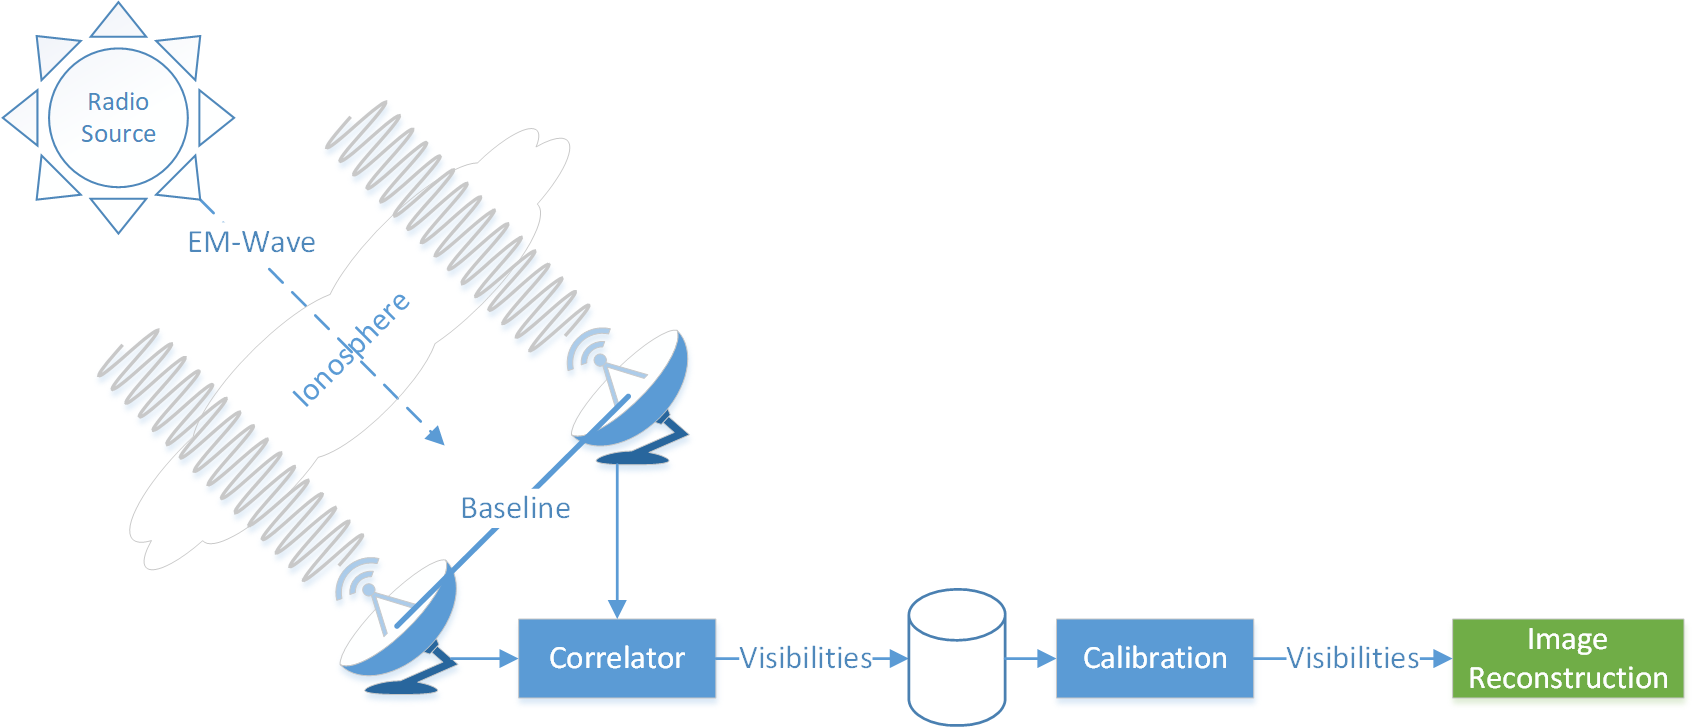
\includegraphics[width=0.80\linewidth]{./chapters/01.intro/system.png}
	\caption{Interferometer System}
	\label{intro:system}
\end{figure}

What Visibilities get measured depends on the antenna layout. The earth rotation modifies the baselines. Due to the earth's rotation, we can sample different Visibilities. (filling the aperture).
Noisy measurements
Only a limited number of Visibilities. This is where the incompleteness comes in. We do not have enough data.
After the Correlator, this is what is saved as the raw measurements.

In the Calibration step, we correct for (Interferometer stuff), Pointing errors, Calibrate the amplitude and phase of the visibilities. Correct for pointing errors. (The interferometer measures relative values). Flagging, remove hopelessly noisy data.
Done before imaging, manual labour.

The last step, the Image Reconstruction is where this work focuses its attention. This is where the ill-posed inverse problem is. We want to find the image corresponding to the calibrated visibilities. 
[Improving the Calibration with partial results of the image reconstruction, done in practice but not part of this project.]
Formally, we want to invert the equation \eqref{intro:inverseproblem}, where $V()$ are the calibrated Visibilities and $I()$ is the observed image. Since the measurements are incomplete, we have many different images $I()$ that fit the Visibilities $V()$, which makes the problem \eqref{intro:inverseproblem} ill-posed.

\begin{equation}\label{intro:inverseproblem}
V(u, v, w) = \int\int \frac{1}{c(x, y)} I(x, y) e^{2 \pi i [ux+vy+ w(c(x, y) - 1)]} \: dx \: dy \quad, \quad c(x,y) = \sqrt{1 - x^2 - y ^2}
\end{equation}

[Not Really 2d Relationship. if $c() << 1$ Fouier part $e^{2 \pi i [ux+vy]}$]. This is the Fourier transform, but in our case we have an extra term $w(c(x, y) - 1)$ that keeps us from using the 2d fourier transform, and by extend the 2d FFT.
But still a linear relationship. Meaning we can express the relationship from Visibilities $V()$ and Image $I()$ with a matrix, which we call $F$. Finding an image is in essence, we try to find a solution to the linear equation \eqref{intro:linear}.

\begin{equation}\label{intro:linear}
FI = V
\end{equation}

Over-determined. In Radio Astronomy, we generally have more Visibilities than Pixels in the reconstruction. At first glance, it seems like we can solve equation \eqref{intro:linear}. 
Why equation \eqref{intro:linear} is ill-posed. 
$F$ is too big for any practical application.
How can we solve this? we need additional information about the image. We find the most likely image $I()$ given the measurements.

How to handle this efficiently.
How can we distribute this.


\subsection{Image Reconstruction}
From the measurements, we want to reconstruct the image, which is the ill-posed inverse problem. Or more formally in equation \eqref{intro:inverseproblem}:

An example is shown in figure \ref{intro:inversefig}.

\begin{figure}[htp]
	% preliminary
	\sbox\twosubbox{%
		\resizebox{\dimexpr.9\textwidth-1em}{!}{%
			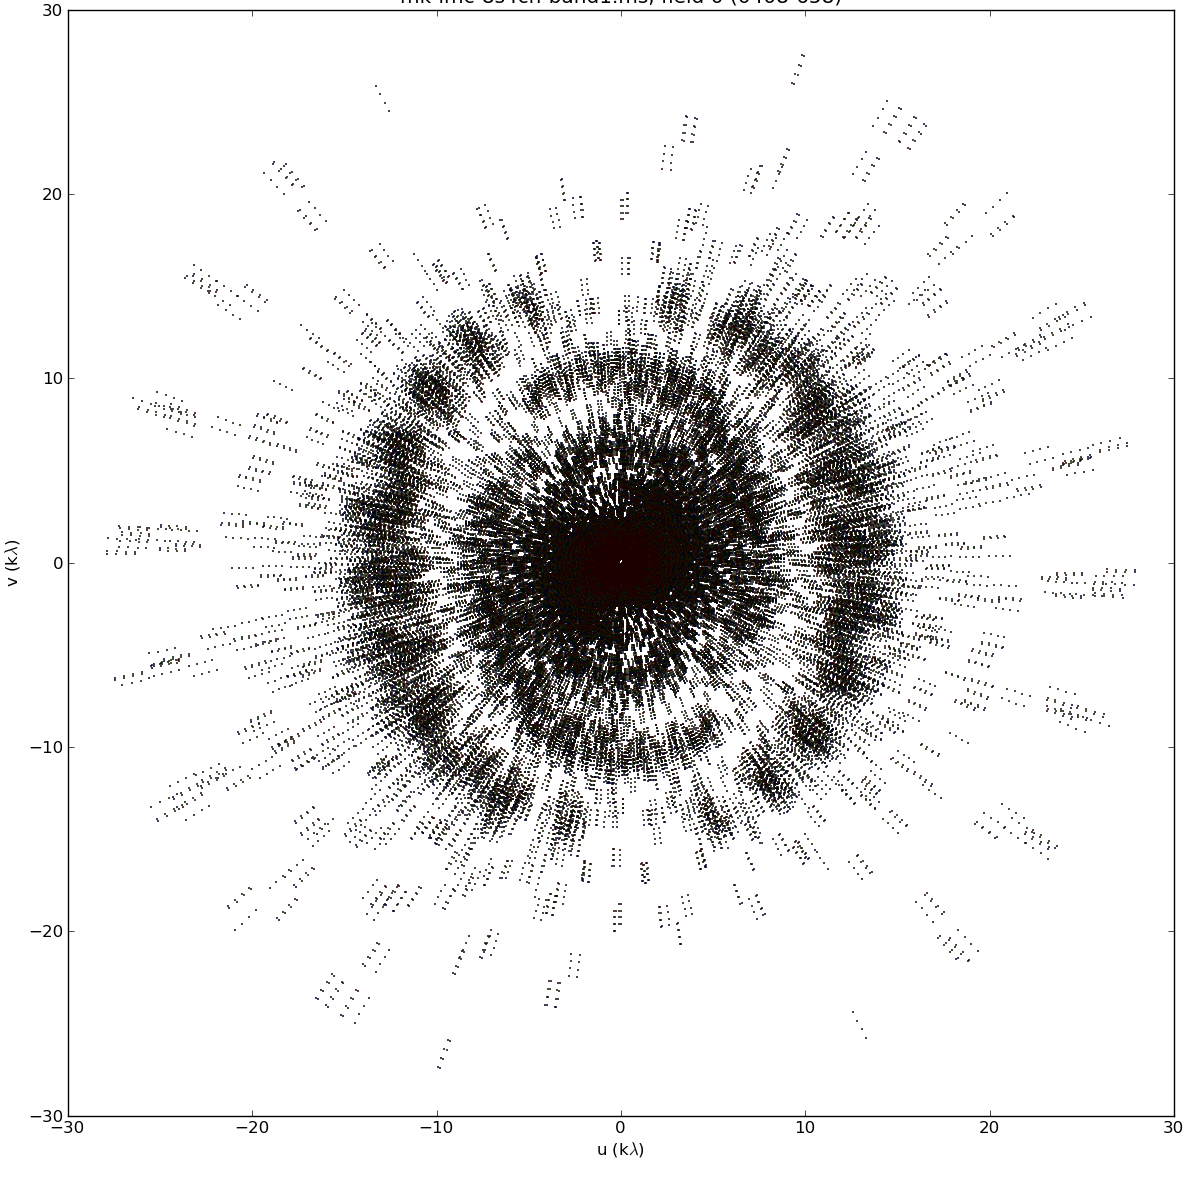
\includegraphics[height=3cm]{./chapters/01.intro/meerkat_uv2.png}%
			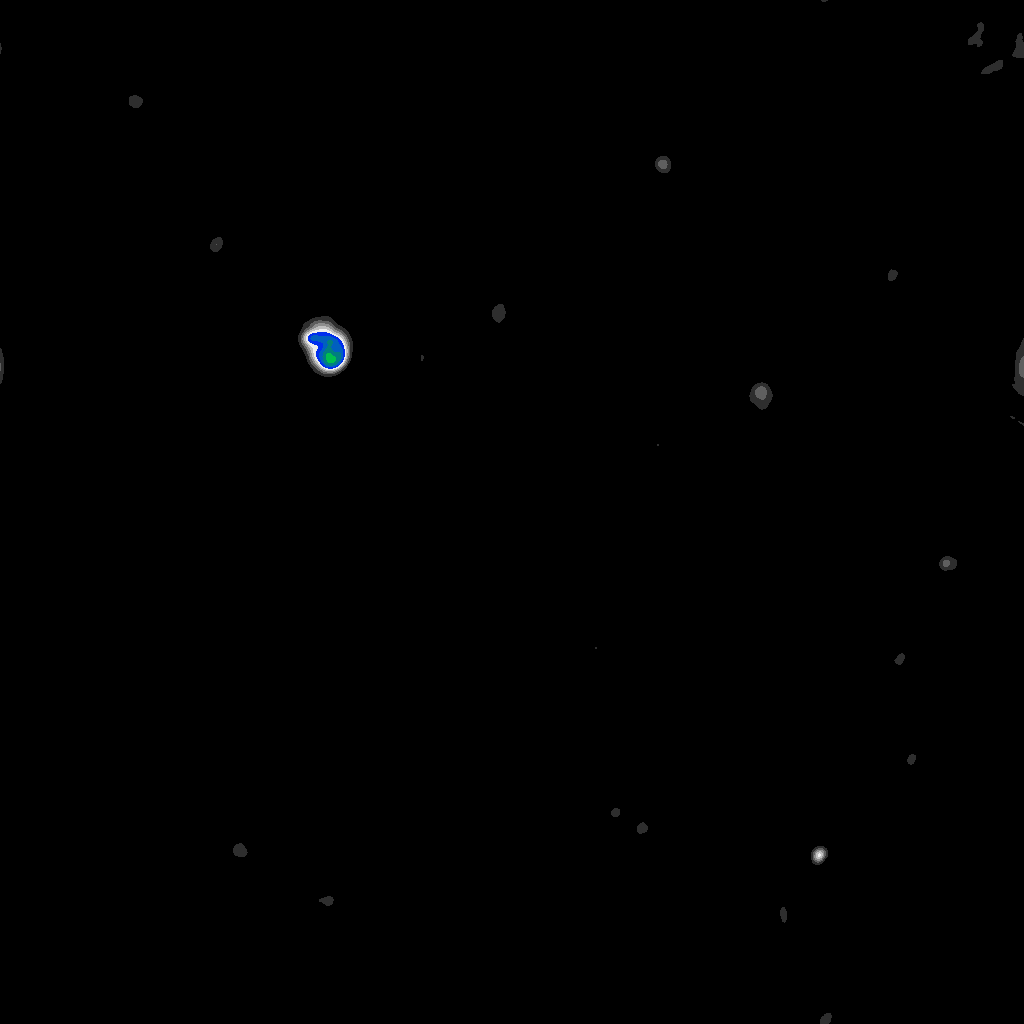
\includegraphics[height=3cm]{./chapters/01.intro/mk2/clean.png}%
		}%
	}
	\setlength{\twosubht}{\ht\twosubbox}
	
	% typeset
	\centering
	\subcaptionbox{Measurements $V()$ in the UV plane.\label{intro:inversefig:uvspace}}{%
		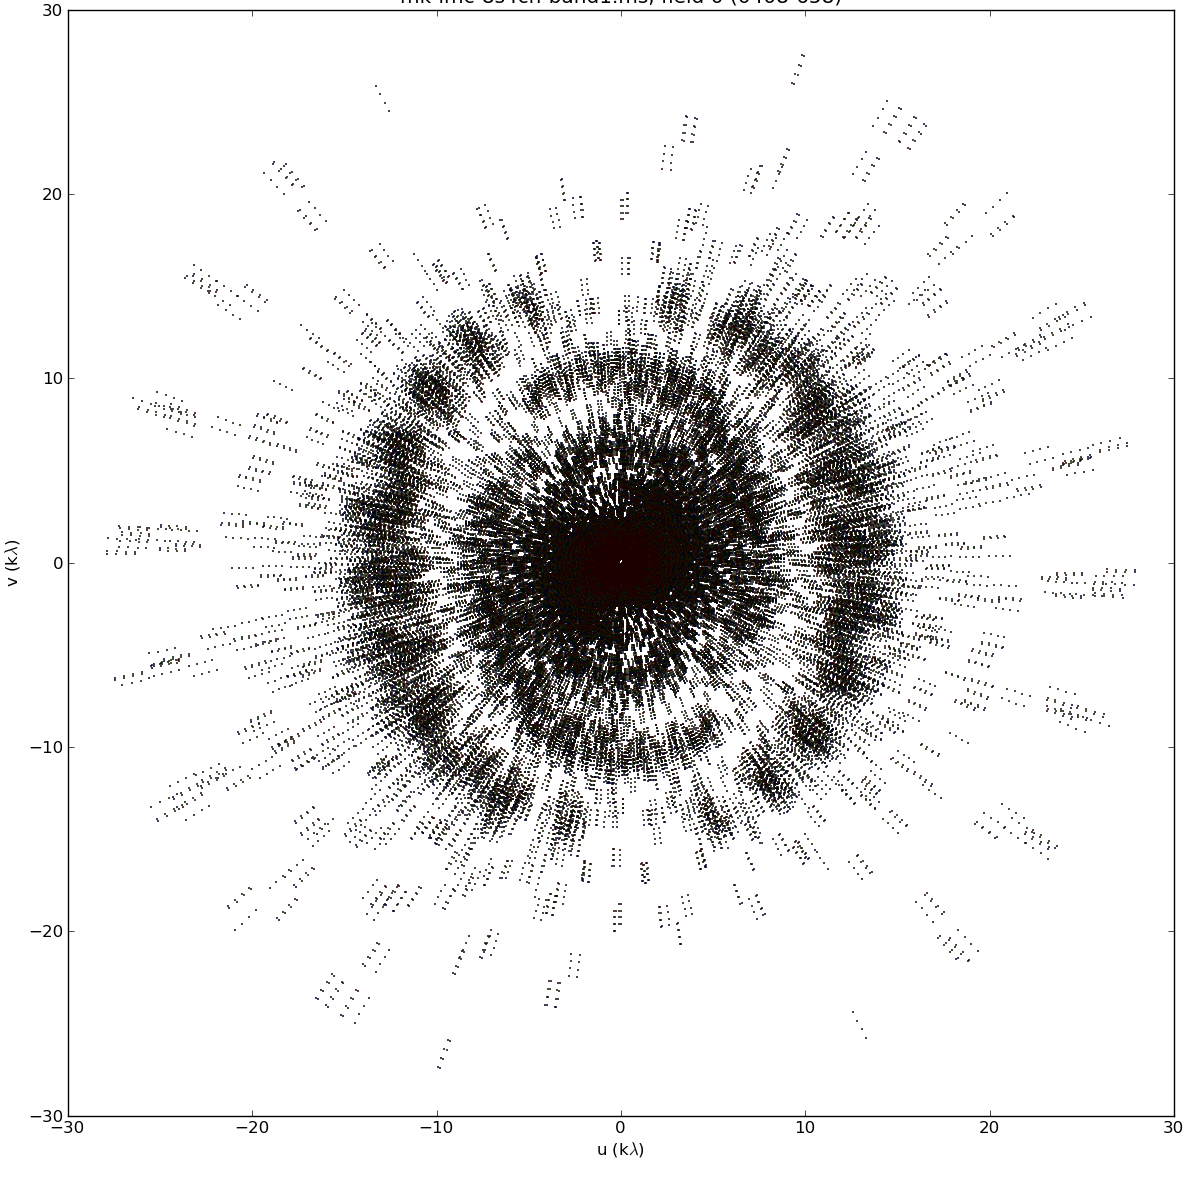
\includegraphics[height=\twosubht]{./chapters/01.intro/meerkat_uv2.png}%
	}\quad
	\subcaptionbox{A reconstructed image $I()$ which fits the measurements.\label{intro:inversefig:reconstruction}}{%
		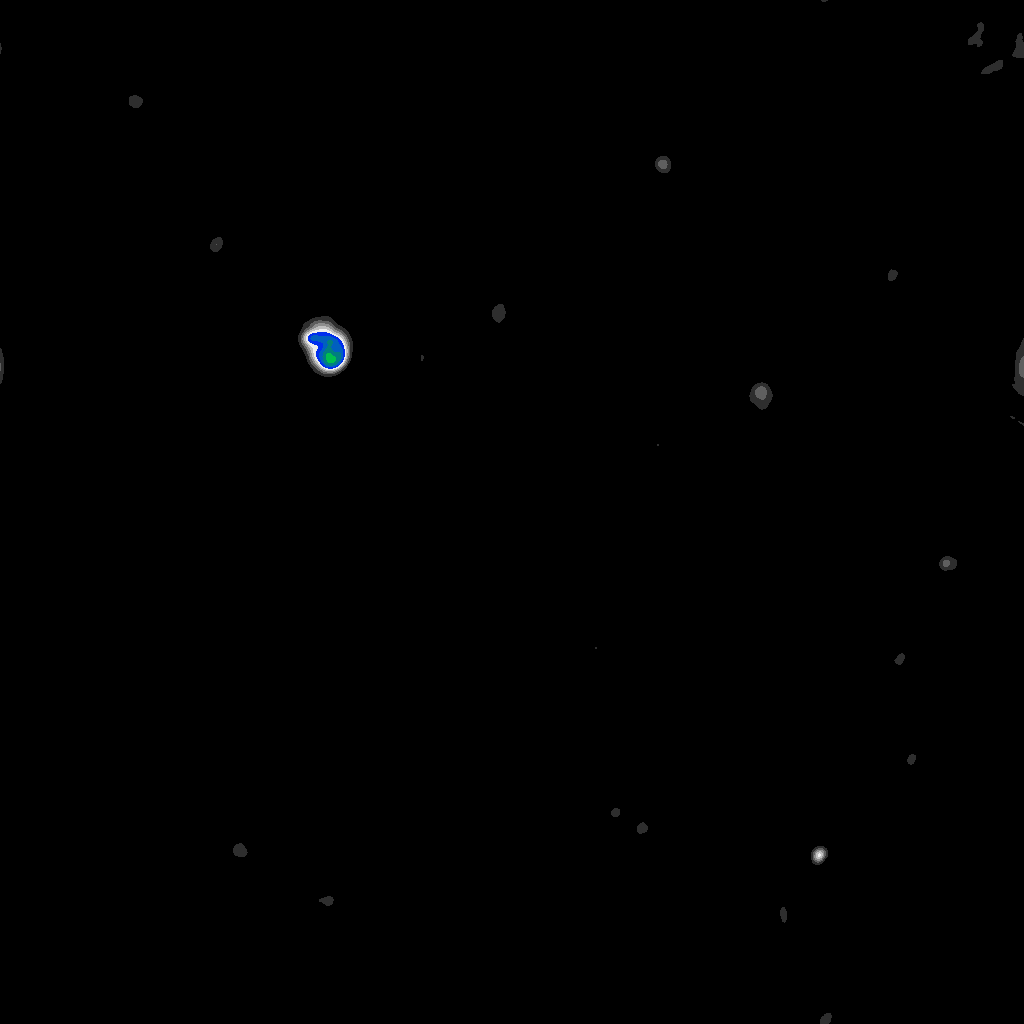
\includegraphics[height=\twosubht]{./chapters/01.intro/mk2/clean.png}%
	}
	\caption{The Image Reconstruction Problem}\label{intro:inversefig}
\end{figure}

The example image shows a few properties of the problem
for $V()$
Incompleteness, holes in the UV space
Continuous space
Non-uniform sampling, we have more densely sampled uv space

For $I()$
Contains two classes of objects: Point sources, which are essentially stars, and extended emissions, which span over several pixels.
Is uniformly sampled
Generally fewer pixels than visibilities
Has bright sources

To transform from $V()$ to $I()$, we have to overcome a few problems.
invert the Almost-Fourier-Equation from \eqref{intro:inverseproblem}. It is not really the 2d Fourier Transform. and as such we cannot use the FFT. How to do this efficiently.
Transform from continuous into discrete space
Into uniformly-sampled space from non-uniform
Lossy Transform


What a high quality reconstruction is. Problem of bright sources in the image
Noise and High dynamic range
So a large part of $V()$ belongs to a few bright sources, but we want to find faint sources "hidden".
image 


\subsubsection{Representation}
Devonbolution vs in-painting.

We do a deconvolution.
Terminology of the dirty image.
\begin{figure}[h]
	\centering
	\begin{subfigure}[b]{0.3\linewidth}
		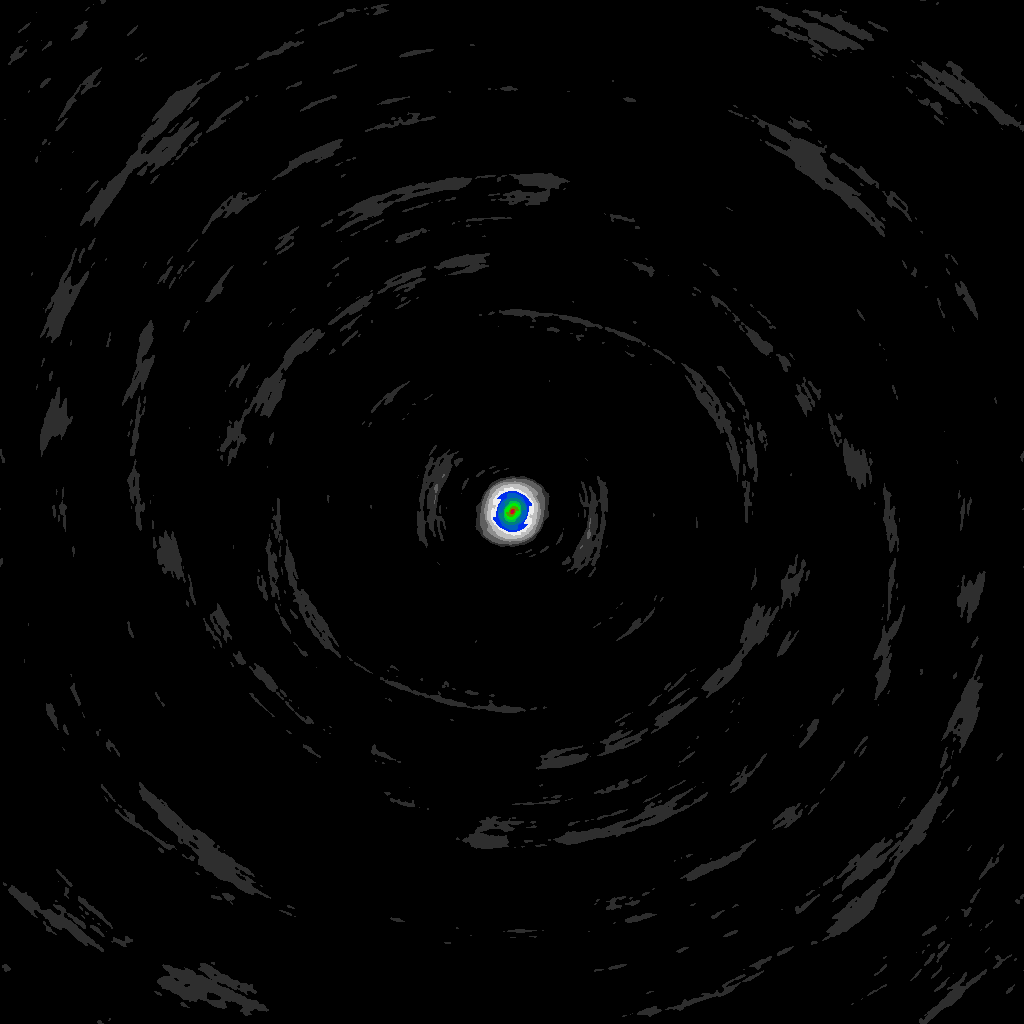
\includegraphics[width=\linewidth]{./chapters/01.intro/mk2/psf.png}
		\caption{Point Spread Function.}
		\label{results:points:tclean}
	\end{subfigure}
	\begin{subfigure}[b]{0.3\linewidth}
		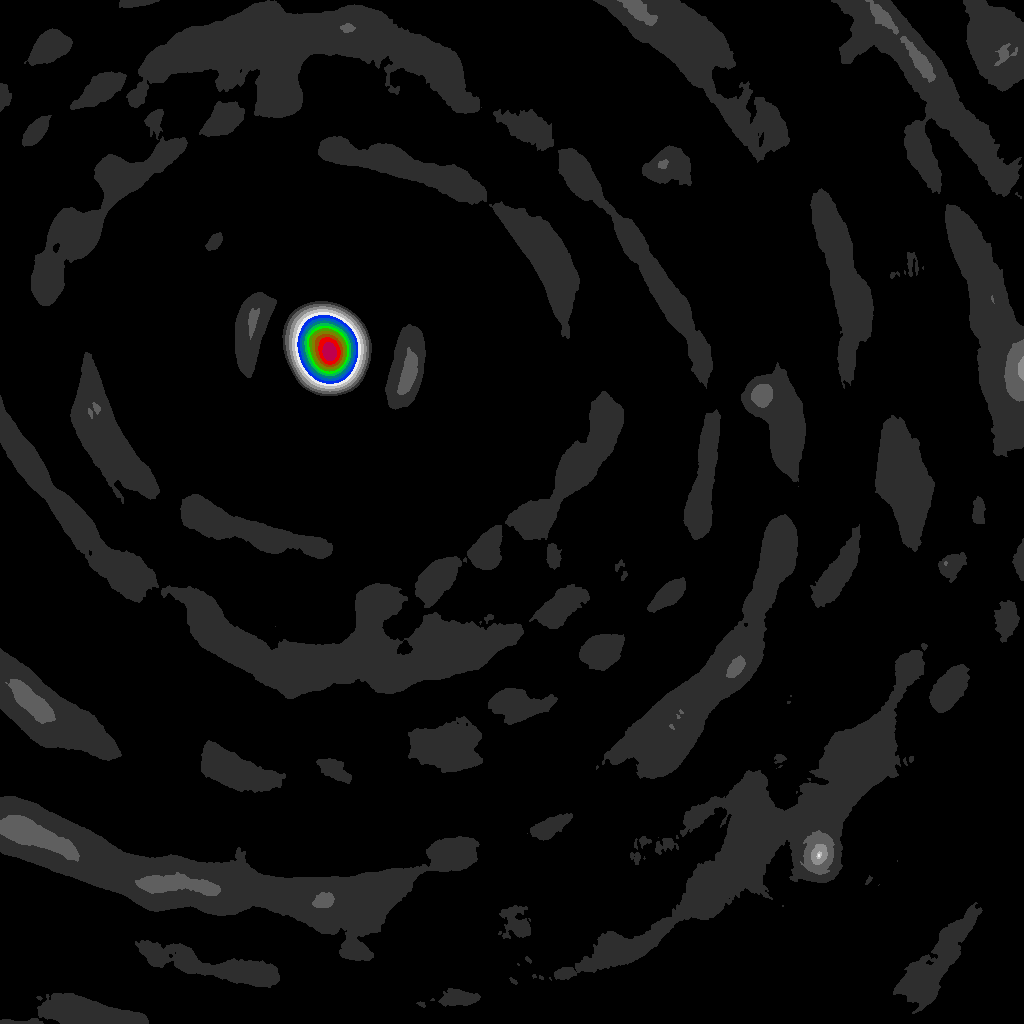
\includegraphics[width=\linewidth]{./chapters/01.intro/mk2/dirty.png}
		\caption{Dirty image}
		\label{results:points:tclean}
	\end{subfigure}
	\begin{subfigure}[b]{0.3\linewidth}
		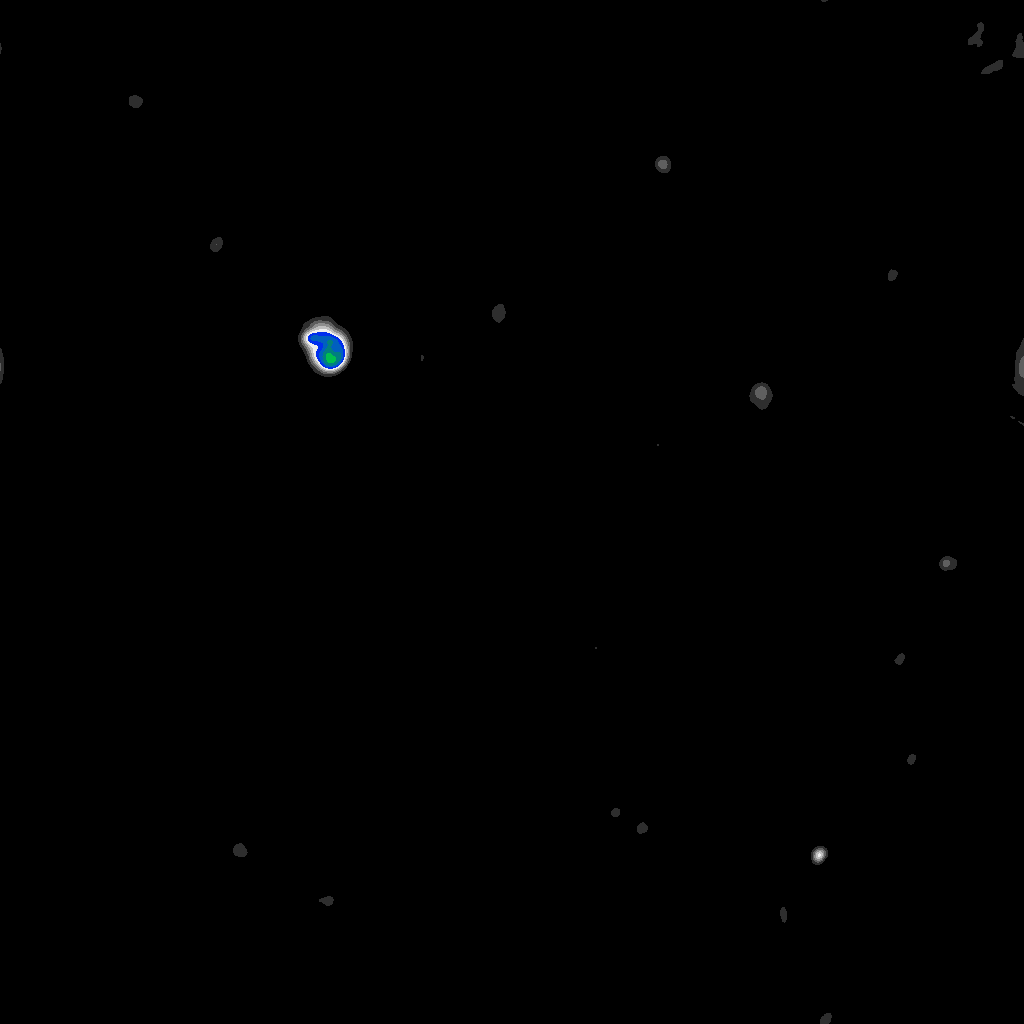
\includegraphics[width=\linewidth]{./chapters/01.intro/mk2/clean.png}
		\caption{Deconvolved image.}
		\label{results:points:tclean}
	\end{subfigure}
	
	
	\caption{Image reconstruction of two simulated point sources.}
	\label{results:points}
\end{figure}




\subsection{The Major Cycle Architecture}
Major cycle how to reconstruct the image with deconvolution
In an efficient manner

$V()$ problems of non-uniform sampling, and the 3 dimensions. keep us from using the Fast Fourier Transform.
We first interpolate on a regularly spaced grid, in the "Gridder".
Use the FFT. For large numbers of Visibilities, this is faster. than inverting equation directly \eqref{intro:inverseproblem}.
And now we do a deconvolution in image space

So we have three basic components, Gridder, FFT and Deconvolution algorithms.
The Major Cycle Architecture makes this a cycle.
Shown in figure \ref{intro:major}.

\begin{figure}[h]
	\centering
	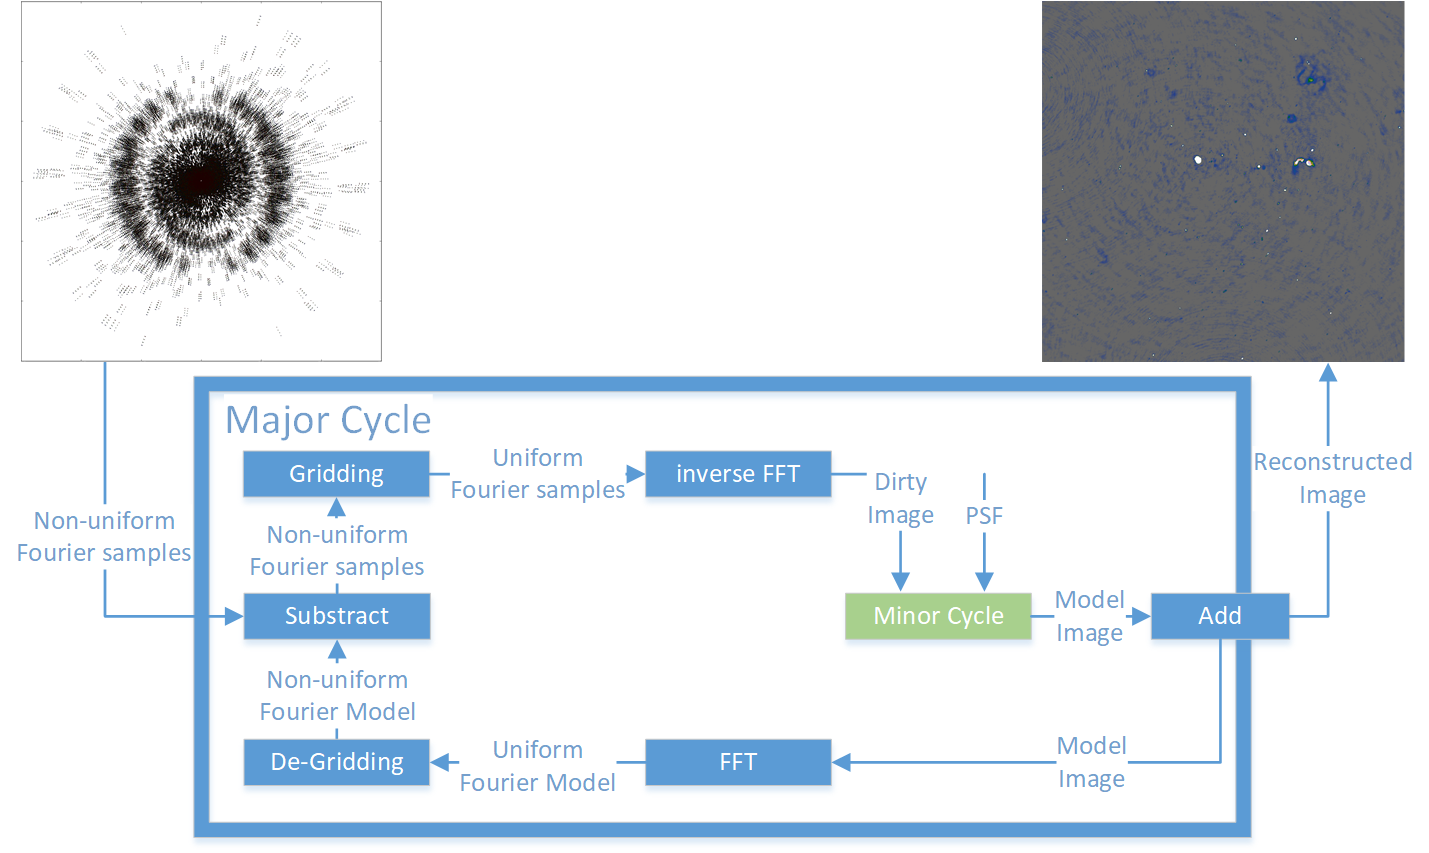
\includegraphics[width=0.80\linewidth]{./chapters/02.hypo/Major-Minor3.png}
	\caption{The Major Cycle Architecture}
	\label{intro:major}
\end{figure}

Why the cycle is necessary
Find the fainter sources in later iterations
Because we can only estimate the psf.


\subsubsection{Minor Cycle}


